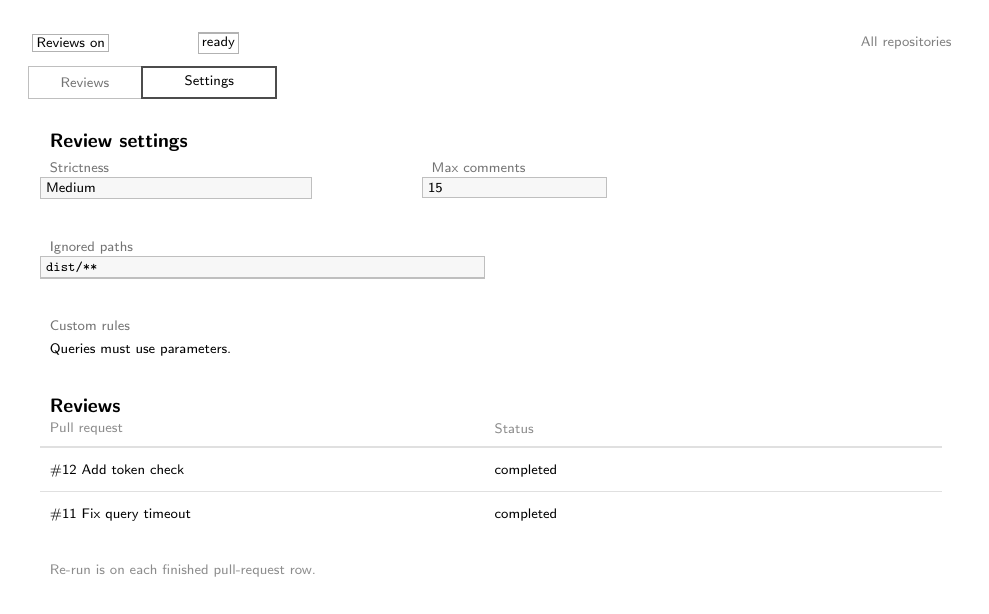
\begin{tikzpicture}[x=1cm,y=1cm]
  \wfchrome{acme/api}{7.25}

  \node[anchor=west, font=\sffamily\tiny, draw=black!30, inner sep=1.4pt] at (3.45,7.55) {Reviews on};
  \node[anchor=west, font=\sffamily\tiny, draw=black!30, inner sep=1.4pt] at (5.55,7.55) {ready};
  \node[anchor=east, font=\sffamily\tiny, text=black!50] at (15.25,7.55) {All repositories};

  % Tabs. Settings is the selected one; the reviews list is drawn below so both are visible.
  \fill[white] (3.40,6.85) rectangle (6.55,7.25);
  \draw[black!25] (3.40,6.85) rectangle (4.85,7.25);
  \draw[black!70, line width=0.7pt] (4.85,6.85) rectangle (6.55,7.25);
  \node[font=\sffamily\tiny, text=black!55] at (4.12,7.05) {Reviews};
  \node[font=\sffamily\tiny] at (5.70,7.05) {Settings};

  \wfpanel{3.40}{3.55}{11.85}{3.15}
  \node[anchor=north west, font=\sffamily\bfseries\scriptsize] at (3.55,6.52) {Review settings};
  \node[anchor=north west, font=\sffamily\tiny, text=black!55] at (3.55,6.15) {Strictness};
  \node[anchor=north west, draw=black!25, fill=black!3, font=\sffamily\tiny, inner sep=2pt, text width=3.3cm] at (3.55,5.85) {Medium};
  \node[anchor=north west, font=\sffamily\tiny, text=black!55] at (8.4,6.15) {Max comments};
  \node[anchor=north west, draw=black!25, fill=black!3, font=\sffamily\tiny, inner sep=2pt, text width=2.2cm] at (8.4,5.85) {15};
  \node[anchor=north west, font=\sffamily\tiny, text=black!55] at (3.55,5.15) {Ignored paths};
  \node[anchor=north west, draw=black!25, fill=black!3, font=\ttfamily\tiny, inner sep=2pt, text width=5.5cm] at (3.55,4.85) {dist/**};
  \node[anchor=north west, font=\sffamily\tiny, text=black!55] at (3.55,4.15) {Custom rules};
  \node[anchor=north west, font=\sffamily\tiny, text width=8cm] at (3.55,3.85) {Queries must use parameters.};

  \wfpanel{3.40}{0.30}{11.85}{3.05}
  \node[anchor=north west, font=\sffamily\bfseries\scriptsize] at (3.55,3.15) {Reviews};
  \node[anchor=west, font=\sffamily\tiny, text=black!45] at (3.55,2.65) {Pull request};
  \node[anchor=west, font=\sffamily\tiny, text=black!45] at (9.2,2.65) {Status};
  \draw[black!12] (3.55,2.42) -- (15.00,2.42);
  \node[anchor=west, font=\sffamily\tiny] at (3.55,2.12) {\#12  Add token check};
  \node[anchor=west, font=\sffamily\tiny] at (9.2,2.12) {completed};
  \draw[black!12] (3.55,1.85) -- (15.00,1.85);
  \node[anchor=west, font=\sffamily\tiny] at (3.55,1.55) {\#11  Fix query timeout};
  \node[anchor=west, font=\sffamily\tiny] at (9.2,1.55) {completed};
  \node[anchor=west, font=\sffamily\tiny, text=black!45] at (3.55,0.85) {Re-run is on each finished pull-request row.};
\end{tikzpicture}
